\documentclass{standalone}

\usepackage{tikz}
\usetikzlibrary{arrows.meta,matrix}
\usepackage{amsmath}

\begin{document}

\begin{tikzpicture}
  \matrix (mat)
  [matrix of nodes,
  nodes={
    anchor=center,
  }]
  {
    Degree
    &$f^{(0)} = \operatorname{id}$
    &$f^{(1)} \circ f^{(0)}$
    & $\dots$
    &$f^{(L)} \circ  \ldots \circ f^{(0)}$
    \\
    0
    & 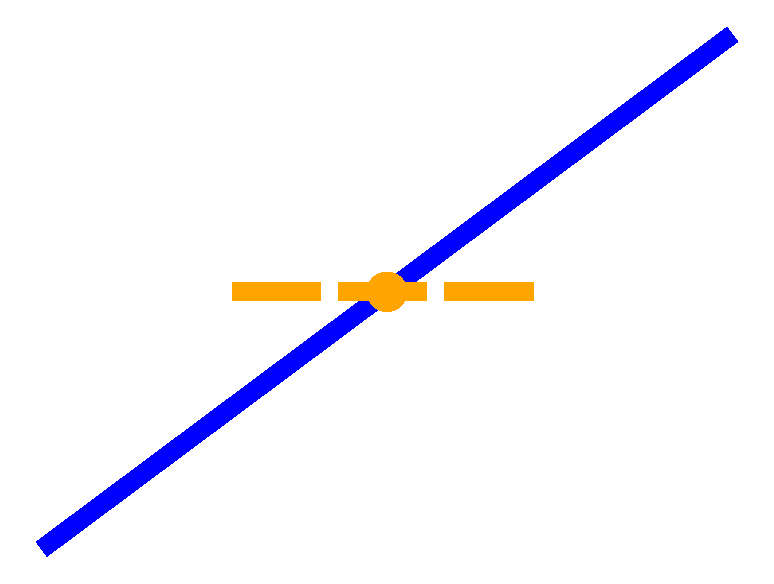
\includegraphics[scale=0.2]{../../kfac_pinns_exp/exp48_visualization_taylor_mode/figures/f_0_taylor_0.pdf}
    & 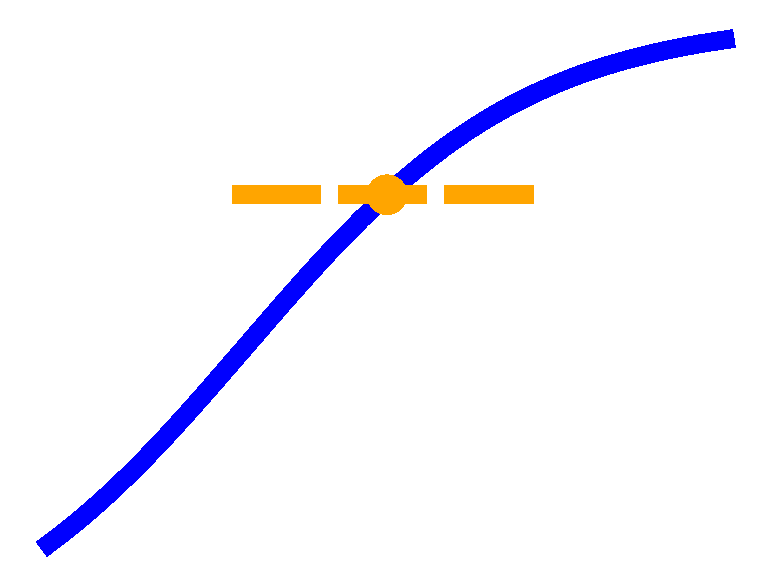
\includegraphics[scale=0.2]{../../kfac_pinns_exp/exp48_visualization_taylor_mode/figures/f_1_taylor_0.pdf}
    & 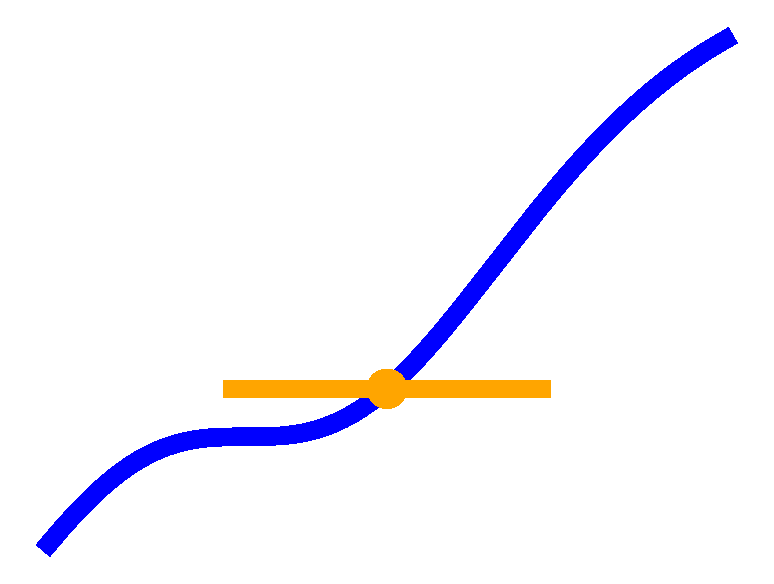
\includegraphics[scale=0.2]{../../kfac_pinns_exp/exp48_visualization_taylor_mode/figures/f_2_taylor_0.pdf}
    & 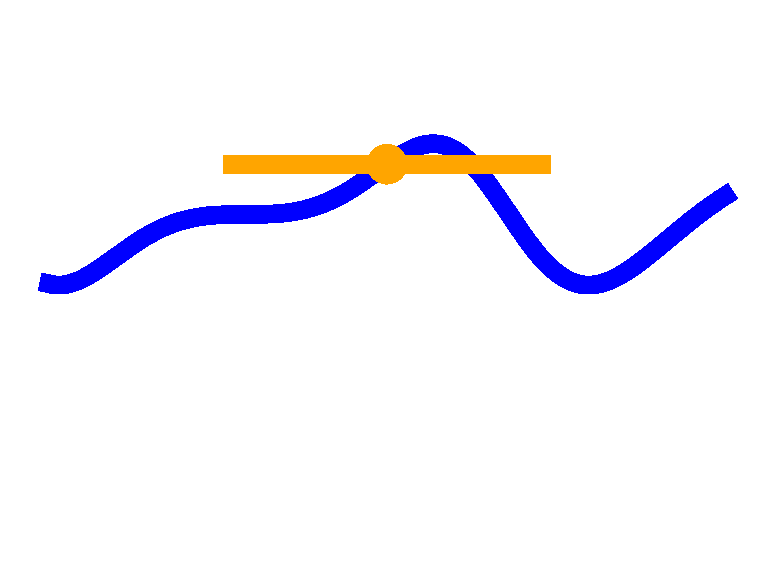
\includegraphics[scale=0.2]{../../kfac_pinns_exp/exp48_visualization_taylor_mode/figures/f_3_taylor_0.pdf}
    \\
    1
    & 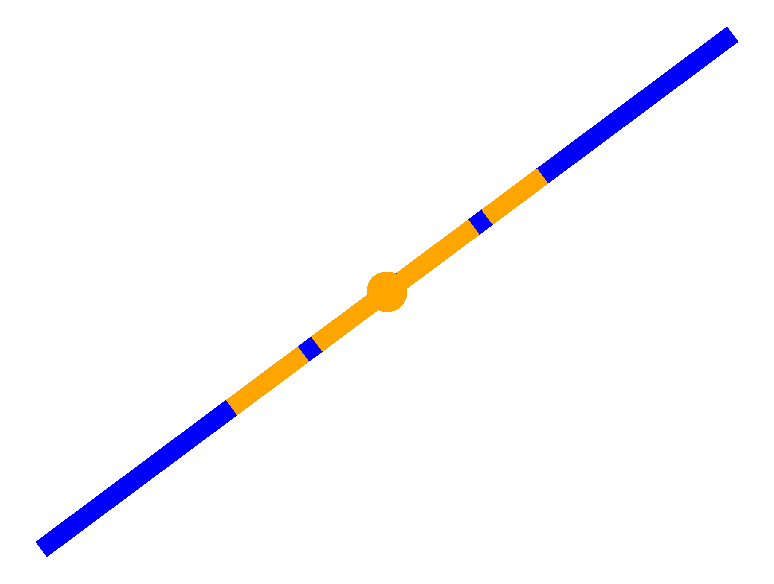
\includegraphics[scale=0.2]{../../kfac_pinns_exp/exp48_visualization_taylor_mode/figures/f_0_taylor_1.pdf}
    & 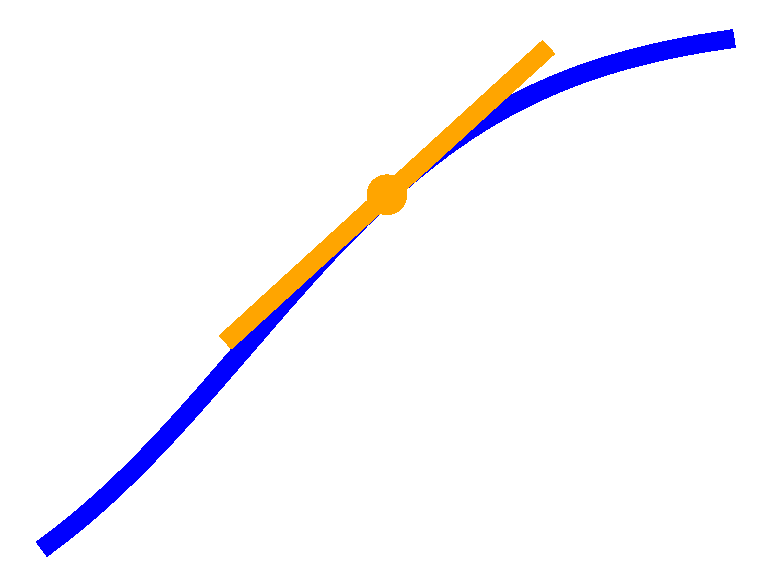
\includegraphics[scale=0.2]{../../kfac_pinns_exp/exp48_visualization_taylor_mode/figures/f_1_taylor_1.pdf}
    & 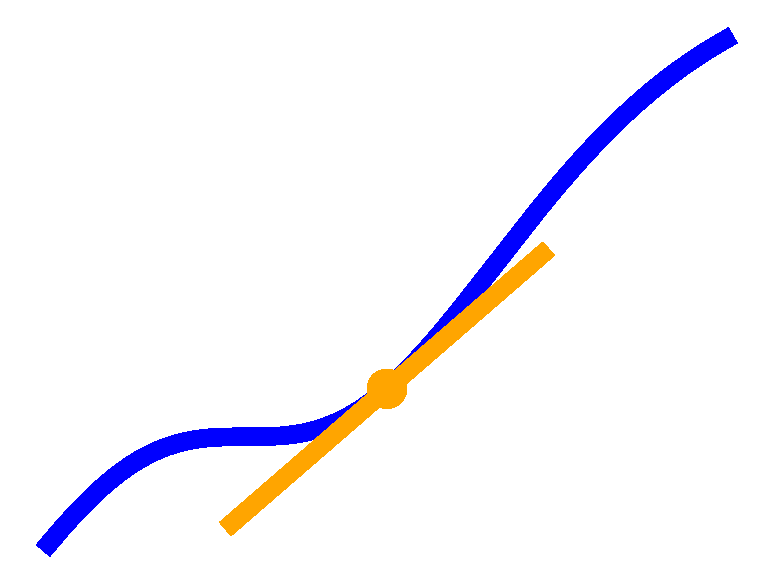
\includegraphics[scale=0.2]{../../kfac_pinns_exp/exp48_visualization_taylor_mode/figures/f_2_taylor_1.pdf}
    & 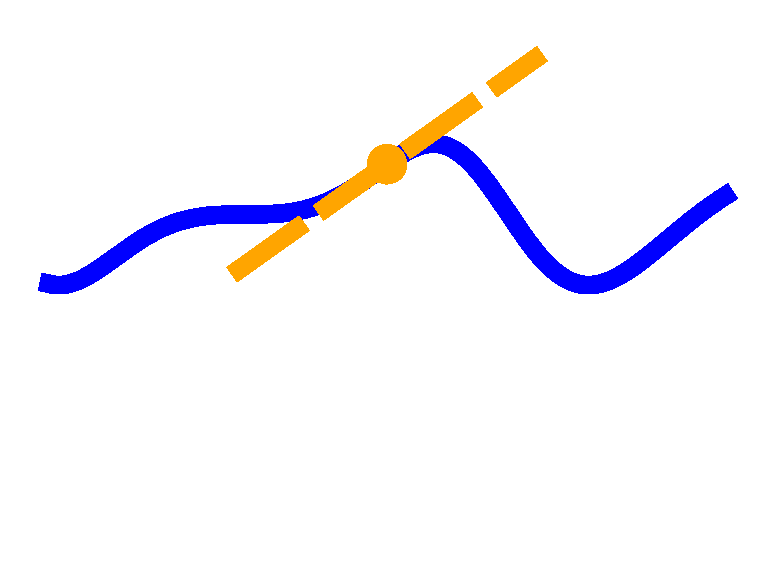
\includegraphics[scale=0.2]{../../kfac_pinns_exp/exp48_visualization_taylor_mode/figures/f_3_taylor_1.pdf}
    \\
    2
    & 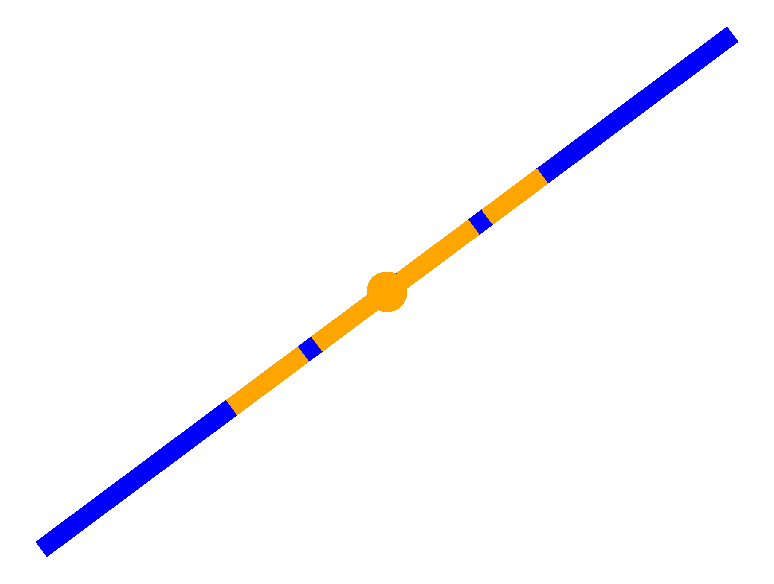
\includegraphics[scale=0.2]{../../kfac_pinns_exp/exp48_visualization_taylor_mode/figures/f_0_taylor_2.pdf}
    & 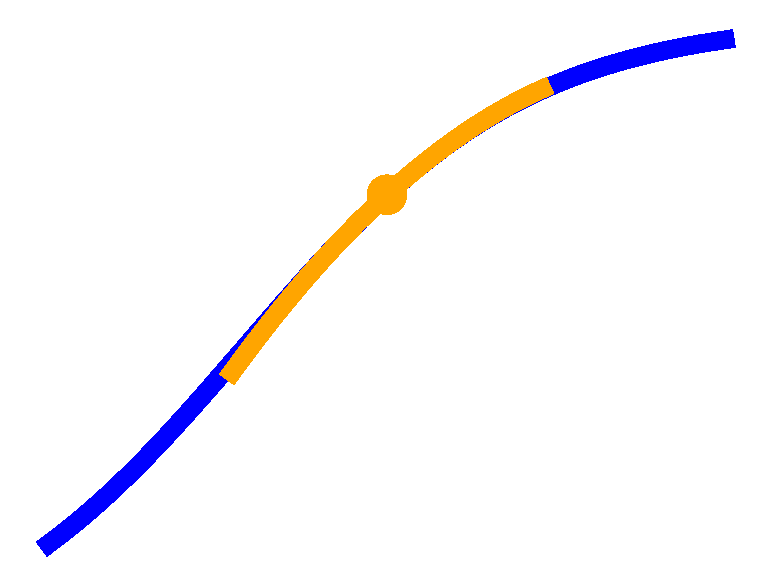
\includegraphics[scale=0.2]{../../kfac_pinns_exp/exp48_visualization_taylor_mode/figures/f_1_taylor_2.pdf}
    & 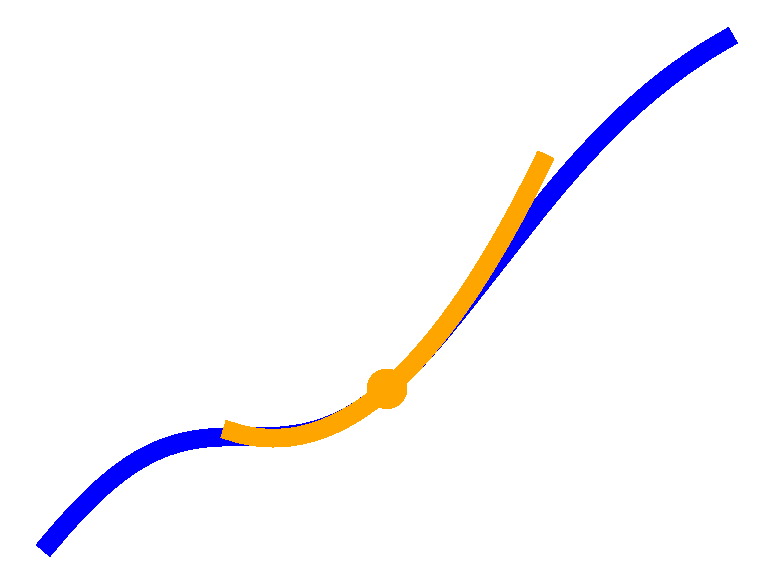
\includegraphics[scale=0.2]{../../kfac_pinns_exp/exp48_visualization_taylor_mode/figures/f_2_taylor_2.pdf}
    & 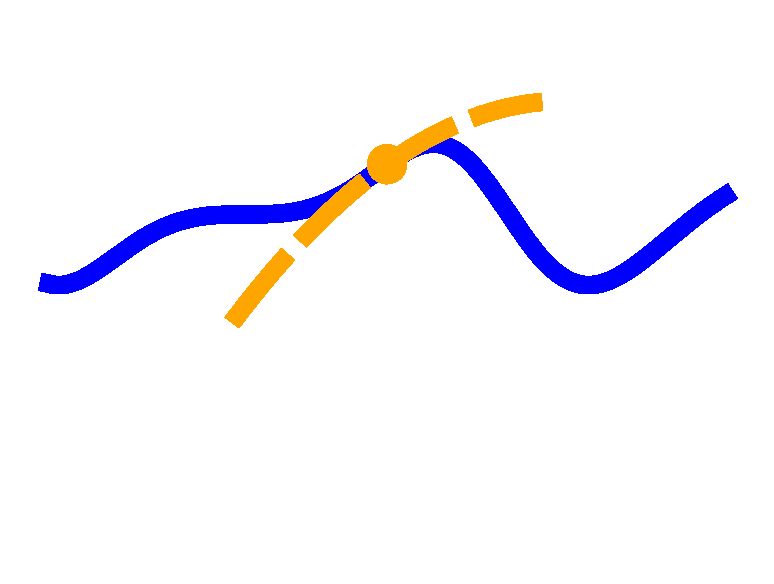
\includegraphics[scale=0.2]{../../kfac_pinns_exp/exp48_visualization_taylor_mode/figures/f_3_taylor_2.pdf}
    \\
    $\vdots$
    & \phantom{$\vdots$}
    &
    &
    & \phantom{$\vdots$}
    \\
  };
  \draw [-Stealth, line width=1.25pt] (mat-5-2) to  node [midway, below] {Propagate} (mat-5-5);
\end{tikzpicture}
\end{document}

%%% Local Variables:
%%% mode: LaTeX
%%% TeX-master: t
%%% End:
